\subsection{Постановка и способы решения чёткой задачи сетевого планирования}

Рассмотрим направленный ациклический граф (DAG, от directed acyclic graph, согласно терминологии~\cite{Kormen}) $G=(V,E)$, $\left| V \right|=n$, $\left| E \right|=m$, обладающий следующими свойствами:
\begin{itemize}
  \item существует ровно одна вершина $v_1\in V$, называемая истоком, из которой рёбра только исходят, т.е. $\forall i=2,n$ $\nexists \left( v_i, v_1 \right)$ ;
  \item существует ровно одна вершина $v_n\in V$, называемая стоком, в которую рёбра графа только входят, т.е.  $\forall i=\overline{1,n-1}$ $\nexists \left( v_n, v_i \right)$;
  \item для любой вершины графа $v_i\in V,\ i=\overline{1,n}$ существует путь $v_1\ldots v_n$, проходящий через неё;
  \item для любого ребра $e_j\in E,\ j=\overline{1,m}$ существует путь $v_1\ldots v_n$, содержащий это ребро.
\end{itemize}

В~задачах календарно-сетевого планирования и управления~(КСПУ) граф, удовлетворяющий перечисленным выше условиям, называется сетевым графиком, и часто применяется для определения продолжительности проекта, состоящего из набора зависящих друг от друга операций~\cite{Kosorukov_Mischenko, Eddous, Taha_Operation_Research, Balashov_IPU}. Обычно работам проекта $w_j$, длительностью $\tau_j$ каждая, сопоставлены дуги графа $e_j$, $j=\overline{1,m}$. Событиям проекта $z_i$ с~временами наступления $t_i$ сопоставления вершины графа $v_i$, $i=\overline{1,n}$. Событие $z_1$~--- начало работ по проекту, событие $z_n$~--- окончание проекта. События проекта (вершины графа) обычно нумеруются, а операции (рёбра) обозначаются словами или буквами латинского алфавита.

Нетрудно заметить, что общее время выполнения проекта $T$ будет равно длине максимального пути в графе, называемого также критическим. Соответственно, операции, которые принадлежат пути максимальной длины, также будут называться критическими. Изменение длительности любой из них приведёт к изменению общего времени выполнения проекта. Остальные операции являются некритическими и характеризуются т.н. резервом времени, т.е. максимальной задержкой по срокам выполнения, при которой общее время проекта не изменится.

Как указано в~\cite{Balashov_IPU}, для сетевого графика всегда существует <<правильная>> нумерация, т.\,е. такая, при которой из вершины с большим порядковым номером не идут дуги в вершину с меньшим порядковым номером. В дальнейшем будем считать, что события проекта перенумерованы так, что нумерация является «правильной».

Для каждого события проекта в~\cite{Eddous, Taha_Operation_Research, Balashov_IPU} определяются следующие понятия.
\begin{mydef}
  Величина $t_{i}^{-}$ называется наиболее ранним моментом наступления события $z_i$ и характеризует момент времени, раньше которого наступление $z_i$ невозможно.
\end{mydef}

\begin{mydef}
  Величина $t_{i}^{+}$ называется наиболее поздним моментом наступления события $z_i$ и характеризует максимальное время наступления $z_i$, при котором общая продолжительность проекта не меняется.
\end{mydef}

\begin{mydef}
  Полным резервом времени для события $z_i$ называется разность наиболее позднего и наиболее раннего моментов его наступления, т.\,е. величина
\begin{equation}
\label{eq:full-event-reserve}
  \Delta t_i=t^+_i-t^-_i.
\end{equation}
\end{mydef}

Для проектных работ в~\cite{Eddous} вводится аналогичное определение.
\begin{mydef}
  Полным резервом времени работы $w_s$, которая начинается при наступлении события $z_{i_s}$ и заканчивается событием $z_{j_s}$, называется величина
\begin{equation}
\label{eq:full-work-reserve}
  \Delta \tau_s=t_{j_s}^{+}-t_{i_s}^{-}-\tau_s.
\end{equation}
\end{mydef}
	
События, у которых полный резерв времени равен нулю, являются потенциально критическими. Соответственно, работа $w_s$ будет считаться критической, если её начальное и конечное событие потенциально критические, а~её общий~резерв времени равен нулю, т.е. одновременно выполняются условия, описываемые формулами~\eqref{eq:full-event-reserve} и~\eqref{eq:full-work-reserve}:
\begin{equation}
\label{eq:critical-work-def}
  \left\{ \begin{aligned}
    & \Delta t_{i_s}=0; \\ 
    & \Delta t_{j_s}=0; \\ 
    & \Delta \tau_s=0.
  \end{aligned} \right.
\end{equation}

Задача поиска критического пути в~графе $G$ может быть решена различными способами, наиболее простым из которых является алгоритмический. Алгоритм поиска критического пути представляет собой алгоритм Дейкстры для~нахождения кратчайшего пути в графе с изменённой функцией релаксации~\cite{Kormen, Indians_CPM}, которая позволяет искать вместо самого короткого пути самый длинный. Каждая вершина графа снабжается двумя метками – временем наиболее раннего наступления события $t_{i}^{-}$ и временем наиболее позднего наступления события $t_{i}^{+}$. В начале работы алгоритма у всех вершин $t_{i}^{-}=0$, $t_{i}^{+}=\infty $. На каждом шаге для вершины $v_i;\ i=\overline{2,n}$ уточняется её $t_{i}^{-}$. Для этого вначале определяются вершины $\left\{ v_j \right\}$, непосредственно предшествующие $v_i$, т.\,е. такие, что существует дуга $e_{ji}$ между $v_j$ и $v_i$. После этого находится $t_{i}^{-}$ путём выбора максимума из сумм $t^{-}$ непосредственно предшествующих событий и длительностей операций, которые связывают каждую из $v_j$ с~$v_i$:
\begin{equation}
\label{eq:earliest-event-time}
  t_{i}^{-}=\underset{v_j}{\mathop{\max }}\,\left\{ t_{j}^{-}+\tau_{ji} \right\}.
\end{equation}

Процесс повторяется до тех пор, пока у всех событий не будут рассчитаны наиболее ранние сроки их наступления. $t_{n}^{-}$ вершины-стока и будет общим временем выполнения проекта. Другими словами,
\begin{equation}
\label{eq:total-project-time}
  T=\underset{i=\overline{1,n}}{\mathop{\max }}\,\left\{ t_{i}^{-} \right\}.
\end{equation}

Если необходимо, помимо общей длительности проекта, отыскать и критический путь, то по графу выполняется обратный проход, во время которого вычисляются наиболее поздние сроки наступления события. Для вершины-стока принимается, что $t_{n}^{+}=t_{n}^{-}$. Для остальных вершин $v_i;\ i=\overline{n-1,1}$ на каждом шаге вначале находятся непосредственно следующие за ними события $\left\{ v_k \right\}$, т.е. такие, что существует дуга $e_{ik}$ между $v_i$ и $v_k$, после чего ищется $t_{i}^{+}$ в виде
\begin{equation}
\label{eq:latest-event-time}
  t_{i}^{+}=\underset{v_k}{\mathop{\min }}\,\left\{ t_{k}^{+}-{{\tau }_{ik}} \right\}.
\end{equation}
Критические операции проекта определяются согласно~\eqref{eq:critical-work-def}.

На рис.~\ref{fig:pplan-crisp} изображён сетевой граф проекта после выполнения вышеописанного алгоритма. Для каждого события проекта указан его номер, наиболее ранний и наиболее поздний сроки его наступления. Пунктиром выделены так называемые фиктивные стрелки (операции) с~нулевой длительностью, которые необходимы для того, чтобы показать зависимость между операциями, не нарушая свойств направленного ациклического графа. Критический путь выделен жирным.
\begin{figure}[h!]
  \centering
  {
    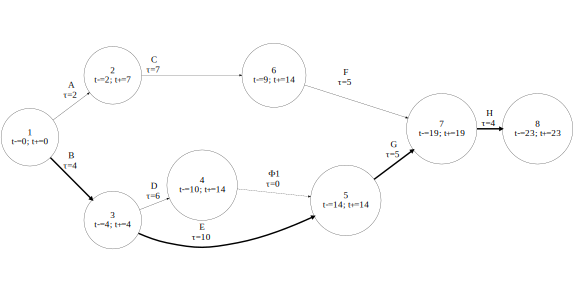
\includegraphics[width=0.9\textwidth]{pplan-crisp}
    \caption{Рассчитанный сетевой график проекта с чёткими временными оценками}
    \label{fig:pplan-crisp}
  }
\end{figure}

К~недостаткам алгоритмического решения стоит отнести трудность исследования задачи на~устойчивость, поскольку результат алгоритмически, а не~аналитически, зависит от~входных данных. Для~исследования на~устойчивость больше подходит решение задачи методами линейного программирования. Классическая постановка этой задачи дана в~\cite{Kosorukov_Mischenko}. Требуется решить задачу
\begin{equation}
\label{eq:crisp-lp-cpm-task}
  T=t_n-t_1 \to \min
\end{equation}
при ограничениях на времена наступления событий
\begin{equation}
\label{eq:crisp-lp-cpm-restrictions}
  t_{j_s}-t_{i_s}\geqslant \tau_s;\ s=\overline{1,m},
\end{equation}
где $t_{i_s}$ и $t_{j_s}$~--- времена наступления событий начала и окончания работы $w_s$ соответственно. Задача~\eqref{eq:crisp-lp-cpm-task} при ограничениях~\eqref{eq:crisp-lp-cpm-restrictions} является задачей линейного программирования.

В~результате решения данной задачи получается общее время выполнения проекта $T$, а также вектор времён $\mathbf{t}=\left\{ t_1, \ldots, t_n \right\}$, называемых календарным планом проекта, и~совокупность критических операций $\mathbf{S}_1$ с нулевым общим резервом времени: $\Delta \tau_{s_1}=0$, $\forall s_1 \in S_1$.

\subsection{Классификация методов решения задачи сетевого планирования с нечёткими параметрами}

Согласно вводимой в~главе~\ref{chapter1} классификации нечётких моделей, в~задаче поиска критического пути источниками нечёткой неопределённости могут быть как параметры (нечёткие времена выполнения операций~\cite{Elizabeth_FCPM}), так и~отношения (нечёткость отношения предшествования операций либо степени включённости операции в проект~\cite{Iran_Morovatdar}). Следуя общей логике диссертации, рассмотрим сформулированные выше задачи~\eqref{eq:total-project-time} и~\eqref{eq:crisp-lp-cpm-task} в~случае, когда для временных оценок длительностей операций используются нечёткие треугольные числа $\tilde \tau_i$ . Решению задачи календарно-сетевого планирования и управления с нечёткими параметрами посвящено немало публикаций в отечественной и зарубежной литературе, однако в большинстве случаев методы её решения можно условно разбить на следующие группы:
\begin{enumerate}
  \item оперирующие нечёткими числами в~неизменной форме с~использованием принципа обобщения. К~этим методам можно отнести, например, описанные в~\cite{Balashov_IPU, Chanas_Zielinski_Criticality, Chanas_Zielinski_FCPM};
  \item вводящие операции сложения, вычитания и~сравнения (либо выбора максимума и~минимума) для нечётких чисел. Подобные методы изложены в~\cite{Uskov_FCPM, Leondes, Dubois_Prade, Iran_Railways};
  \item использующие дефаззификацию или получение чётких $\alpha$-уровневых значений. Такие методы, описанные в~\cite{Egyptians, Indians_FCPM, Chinese_CPM}, обычно основываются на~линейном программировании;
  \item комбинированные методы, описанные, например, в~\cite{Liang_Han_FCPM}.
\end{enumerate}

Рассмотрим методы первой группы на примере решения задачи поиска критического пути в~\cite{Balashov_IPU}. Пусть заданы функции принадлежности для нечётких~оценок продолжительности операций $\mu_{\tilde \tau_s}\left( x \right)$. Если за $Q_i$ обозначить множество номеров вершин, непосредственно предшествующих вершине $v_i$, a за $R_i$~--- множество номеров вершин, непосредственно следующих за $v_i$, то, согласно принципу обобщения Заде, функция принадлежности нечёткого наиболее раннего срока наступления события $z_i$ имеет вид
\begin{equation}
\label{eq:fcpm-zadeh-earliest}
  \mu_{\tilde{t}_{i}^{-}}\left( x \right)=\underset{\left\{ \left( x_{ji} \right),j\in Q_i \left| \max \left( x_j+x_{ji} \right)=x \right. \right\}}{\mathop{\max }}\,\min \left[ \underset{j\in Q_i}{\mathop{\min }}\,\left( \mu_{\tilde{t}_{ji}^{-}}\left( x_{ji} \right) \right);{\mu_{\tilde{t}_{j}^{-}}}\left(x_j \right) \right].
\end{equation}
Функция принадлежности наиболее позднего срока наступления вычисляется следующим образом:
\begin{equation}
  \mu_{\tilde{t}_{i}^{+}}\left( x \right)=\underset{\left\{ \left( T,x_i \right)\left| T-x_i=x \right. \right\}}{\mathop{\max }}\,\underset{i=\overline{1,n}}{\mathop{\min }}\,\left[ \mu_{\tilde T}\left( T \right);\mu_{\tilde l_i}\left(x_i \right) \right],
\end{equation}
где $\tilde l_i$~--- нечёткая максимальная длина пути от вершины $v_i$ до стока $v_n$, определяемая через функцию принадлежности
\begin{equation}
  \mu_{\tilde l_i}\left( x \right)=\underset{\left\{ \left(x_{ij} \right),j\in R_i\left| \max \left( x_j+x_{ji} \right)=x \right. \right\}}{\mathop{\max }}\,\min \left[ \underset{j\in R_i}{\mathop{\min }}\,\left( \mu_{\tilde t_{ij}}\left( x_{ij} \right) \right);\mu_{\tilde l_j}\left(x_j \right) \right],
\end{equation}
a $\tilde T$ – общее время проекта, функция принадлежности которого рассчитывается как
\begin{equation}
  \mu_{\tilde T}\left( T \right)=\underset{\left\{ \left(x_i \right),i=\overline{1,n}\left| \min \left(x_j \right)=T \right. \right\}}{\mathop{\max }}\,\underset{j=\overline{1,n}}{\mathop{\min }}\,\left( \mu_{\tilde{t}_{j}^{-}}\left(x_j \right) \right).
\end{equation}
Функции принадлежности полных нечётких резервов времени для событий имеют вид
\begin{equation}
\label{eq:fcpm-event-reserves}
  \mu_{\Delta \tilde{t}_i}\left( x \right)=\underset{\left\{ \left( y_i, x_i \right)\left| y_i-x_i=x \right. \right\}}{\mathop{\max }}\,\min \left[ \mu_{\tilde{t}_{i}^{+}}\left(y_i \right); \mu_{\tilde{t}_{i}^{-}}\left(x_i \right) \right].
\end{equation}
	
В полученной модели, задаваемой формулами~\eqref{eq:fcpm-zadeh-earliest}--\eqref{eq:fcpm-event-reserves}, нельзя однозначно указать, какое из событий является критическим~---авторы~\cite{Balashov_IPU} указывают, что функции принадлежности полных резервов времени для каждого события~\eqref{eq:fcpm-event-reserves} при $x=0$ могут быть интерпретированы как степени принадлежности событий критическому пути. В~\cite{Balashov_IPU} также предлагается следующая классификация событий для~модели КСПУ с~интервальной неопределённостью~--- критические, полукритические и~некритические. Согласно результатам, полученным в~\cite{Chanas_Zielinski_Criticality}, схожая классификация может быть распространена и на нечёткий случай:
\begin{itemize}
  \item однозначно критической в~\cite{Chanas_Zielinski_Criticality} называется такая операция, которая при замене длительностей операций $\tilde \tau_i$ во всём проекте их любыми чёткими значениями $\tau_i\in supp\left( \tilde \tau_i \right)$ является критической в классическом понимании этого термина;
  \item потенциально некритической называется такая операция, которая при замене длительностей операций $\tilde \tau_i$ во всём проекте их любыми чёткими значениями $\tau_i\in supp\left( \tilde \tau_i \right)$, не является критической в классическом понимании этого термина.
\end{itemize}

Решение задачи, предложенное в~\cite{Balashov_IPU}, обладает несколькими существенными недостатками:
\begin{itemize}
  \item громоздкость вычислений, основанных на принципе обобщения Заде;
  \item как отмечено в~\cite{Chanas_Zielinski_Criticality}, до сих пор остаётся нерешённым в общем случае вопрос о степени критичности операции из-за трудности нахождения отдельных критических операций в сетях проектов, где не существует однозначно критического пути, т.\,е. такого, все операции которого являются однозначно критическими;
  \item сложность интерпретации результата лицом, принимающим решение~--- трудно выбрать из~нескольких критических путей <<наиболее критический>>, в~\cite{Chanas_Zielinski_Criticality} для этого используется довольно громоздкий алгоритм;
  \item не~решена проблема устойчивости решения~--- применение принципа обобщения может привести к~неоправданному расширению носителя результата, что~также сказывается на~полезности его практического применения.
\end{itemize}

Методы, использующие результаты нечётких арифметик, рассмотрим на примере задачи поиска критического пути в~проекте с~нечёткими времнными оценками из~\cite{Dubois_Prade}. При решении задачи используется описанный выше для чёткого случая модифицированный алгоритм Дейкстры. Операции сложения и~вычитания, необходимые в~\eqref{eq:earliest-event-time} и~\eqref{eq:latest-event-time}, определяются через принцип обобщения Заде согласно~\eqref{eq:zadeh-algebra} (в~\cite{Iran_Railways, Uskov_FCPM, Leondes} для арифметических операций используются правила работы с~нечёткими LR-числами). Расширенная операция <<максимум>> для двух нечётких LR-чисел в~\cite{Dubois_Prade, Uskov_FCPM} определяется как
\begin{equation*}
  \max \left(\tilde A, \tilde B \right) = \left(m; a; b \right),
\end{equation*}
где $m$, $a$, $b$ определяются согласно формуле
\begin{equation}
  \label{eq:fcpm-dubois-max}
  \left \{ \begin{aligned}
    & m = \max \left( m_{\tilde A}, m_{\tilde B} \right); \\
    & a = \max \left( m_{\tilde A}, m_{\tilde B} \right) - \max \left( m_{\tilde A} - a_{\tilde A}, m_{\tilde B} - a_{\tilde B} \right); \\
    & b = \max \left( m_{\tilde A} + b_{\tilde A}, m_{\tilde B} + b_{\tilde B} \right) - \max \left( m_{\tilde A}, m_{\tilde B} \right).
  \end{aligned} \right.
\end{equation}
а~операция <<минимум>> получается с~помощью замены $\max$ на~$\min$ в~выражении~\eqref{eq:fcpm-dubois-max}.

Методы второй группы обычно позволяют решать задачу поиска времени выполнения проекта с~помощью стандартного ПО, однако при этом их применимость ограничена ввиду следующих недостатков:
\begin{itemize}
  \item алгоритмы решения задачи получают проблемы в~наследство от~используемых в~них определений нечёткой арифметики, а~итоговые результаты (время выполнения и критический путь) сильно зависят от~вводимых операций максимума/минимума либо используемого способа сравнения нечётких чисел;
  \item в~процессе вычислений могут возникать лишённые физического смысла отрицательные времена наступления событий, как, например, в~\cite{Liang_Han_FCPM};
  \item в~\cite{Leondes, Zielinski_Preprint} приводятся примеры, иллюстрирующие тот факт, что при непосредственном использовании нечётких чисел иногда нельзя выполнять обратный проход по~сети проекта для поиска критического пути, поскольку есть риск учесть нечёткость времён выполнения операций дважды при выборе минимума и~вычитании согласно~\eqref{eq:latest-event-time}. В~связи с~этим, после обратного прохода наиболее поздние сроки наступления событий будут максимально размытыми.
\end{itemize}

$\alpha$-уровневые методы и методы, использующие дефаззификацию, рассмотрим на~примерах из~\cite{Indians_FCPM} и~\cite{Chinese_CPM}. В~статье~\cite{Chinese_CPM} задача поиска критического пути сводится к~вычислению индексов ранжирования Ягера для каждой из нечётких оценок $\tilde \tau_{ij}$, $v_i,v_j \in V$:
\begin{equation*}
  I\left(\tilde \tau \right) = \int \limits_{0}^{1}{\frac{1}{2}\left(x^L \left(\alpha \right)+x^R \left(\alpha \right) \right) d\alpha},
\end{equation*}
которые затем используются в~задаче целочисленного программирования
\begin{equation}
\label{eq:yager-ranking-lp-cpm}
  I \left( \tilde T \right) = \sum \limits_{i=1}^{n}\sum \limits_{j=1}^{n} I\left(\tilde \tau_{ij} \right)x_{ij} \to \max
\end{equation}
с ограничениями
\begin{equation}
\label{eq:lp-cpm-int-constraints}
  \left \{ \begin{aligned}
    & \sum \limits_{j=1}^n x_{1j}=1; \\
    & \sum \limits_{j=1}^n x_{ij}= \sum \limits_{k=1}^n x_{ki},\ i=\overline {2, n-1}; \\
    & \sum \limits_{k=1}^{n} x_{kn}=1; \\
    & x_{ij} \geqslant 0,
  \end{aligned} \right.
\end{equation}
где $x_{ij}$ обозначает величину потока, проходящего через дугу $e_{ij}$. Решением задачи~\eqref{eq:yager-ranking-lp-cpm} является время выполнения проекта $\displaystyle \tilde T = \sum \limits_{i=1}^{n} \sum \limits_{j=1}^{n} \tilde \tau_{ij} x_{ij}$ и~соответcтвующий ему путь $p^*$. Для всех остальных путей графа $p_k$, $k=\overline{1,m}$ от истока к стоку находится их степень критичности согласно формуле~\eqref{eq:path-criticality-degree}:
\begin{equation}
\label{eq:path-criticality-degree}
  deg_{Cr}\left(p_k \right) = \frac{\sum \limits_{i=1}^{n} \sum \limits_{j=1}^{n} I\left(\tilde \tau_{ij} \right) x_{ij}^{p_k}}{\sum \limits_{i=1}^{n} \sum \limits_{j=1}^{n} I\left( \tilde \tau_{ij} \right) x_{ij}^{p^*}}.
\end{equation}

Предлагаемая в~\cite{Indians_FCPM} методика решения отличается от вышеописанной тем, что величина потока также выражается нечётким числом $\tilde x_{ij}$; её вариант, изложенный в~\cite{Kumar_FCPM_Triangular} оперирует нечёткими числами в~форме, позволяющей сократить число условий и параметров в задаче линейного программирования; а в~\cite{Egyptians, Chen_CPM} задача поиска критического пути рассматривается как задача двухуровневой оптимизации~--- на каждом $\alpha$-уровне решается вначале задача поиска верхней (правой) границы $\alpha$-интервала с~ограничениями~\eqref{eq:lp-cpm-int-constraints}:
\begin{equation*}
  \tilde T^R \left( \alpha \right) = \sum \limits_{i=1}^{n} \sum \limits_{j=1}^{n} I\left(\tilde \tau_{ij}^R \left(\alpha \right) \right)x_{ij} \to \max,
\end{equation*}
после чего решается двойственная ей задача по поиску нижней (левой) границы $\alpha$-интервала
\begin{equation*}
  \tilde T^L \left( \alpha \right) = y_n-y_1 \to \min
\end{equation*}
с~ограничениями, аналогичными~\eqref{eq:crisp-lp-cpm-restrictions}:
\begin{equation*}
  y_j-y_i \geqslant \tau_{ij}\left( \alpha \right),\ i,j=\overline{1, n}.
\end{equation*}

Методы третьей группы позволяют решать задачу поиска нечёткого критического пути максимально независимо от форм функций принадлежности числовых параметров. Среди потенциальных проблем этих методов можно выделить следующие:
\begin{itemize}
  \item выбор неподходящего индекса ранжирования для нечётких параметров, а также наличие потенциально несравнимых временных оценок;
  \item сложности при восстановлении функции принадлежности нечёткого результата по~значениям на~различных $\alpha$-уровнях.
\end{itemize}